\section{User Interface}

\subsection{Web-Based Front-end}

The web-based front-end of OpenPRA is designed to address the existing gaps in the current ecosystem of \acrshort{pra} tools. The front-end tries to meet a comprehensive set of requirements demanded by evolving technological landscape, including:

\begin{itemize}
\item \textbf{User friendly interface:} Provides an intuitive, browser-based \acrshort{ui} with built-in visualization tools, lowering the barrier for users of all technical backgrounds.
\item \textbf{Web based access:} Allows secure access via \acrshort{https} without client installation, supporting remote workflows.
\item \textbf{Open source platform:} Freely available and community‑driven, promoting transparency, collaboration, and continuous improvement.
\item \textbf{Collaborative environment:} Enables multiple users to work concurrently on the same \acrshort{pra} model, improving teamwork and efficiency across multiple teams.
\item \textbf{Version control:} Records changes to a model, persists revision history, and supports version rollback whenever a prior state must be restored.  
\item \textbf{Support for a wide range of risk models:} Provides editors for event trees, fault trees, Markov chains, Bayesian networks, and other formalisms, enabling analysts to choose a risk model that best represents their system.  
\item \textbf{Choice of quantification engines:} Integrates multiple built‑in and third‑party solvers so analysts can select an algorithm most suitable for their use case.  
\item \textbf{Interoperability:} Serializes models to the standardized OpenPRA \acrshort{mef} \acrshort{json} format, ensuring seamless data exchange with external tools and workflows.
\item \textbf{Customizability:} Allows users to tailor the interface, workflows, and analysis parameters to their specific project requirements.
\end{itemize}

\begin{figure}[h!]
  \centering
  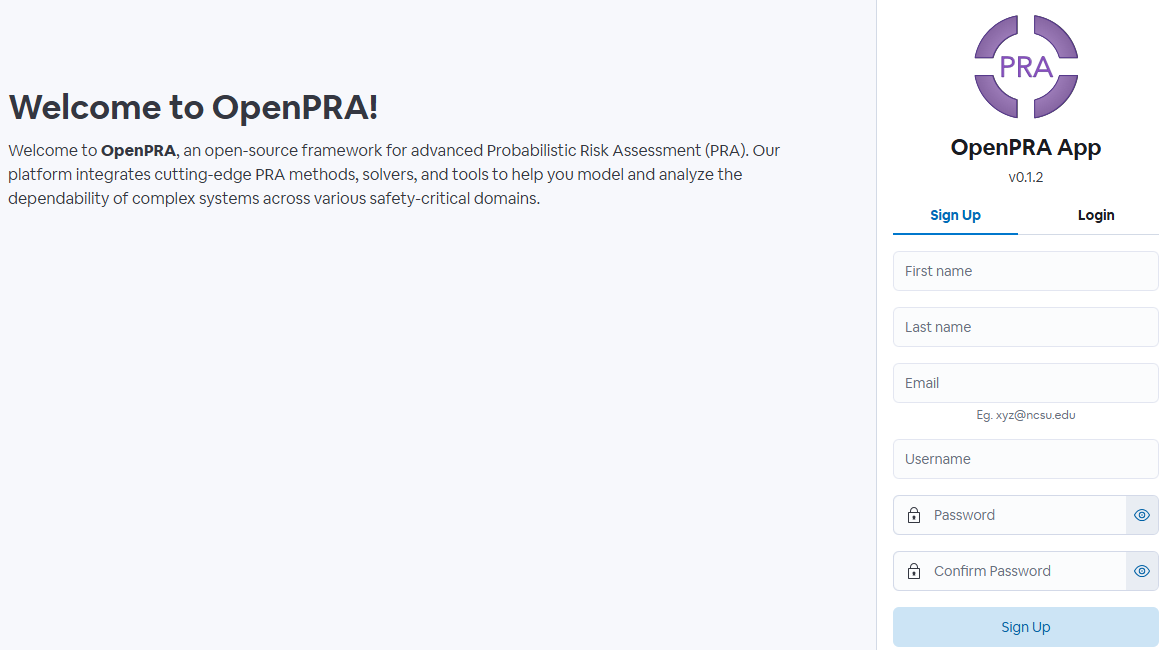
\includegraphics[width=0.9\textwidth]{4_proposed_solution/web_app/figures/landing_page.png}
  \caption{Landing page of the OpenPRA web application.}
  \label{fig:landing_page}
\end{figure}

\subsection{Analysis Modes, Types and Risk Models}

The front-end supports a wide range of analysis modes, analysis types and risk models. This enables users to tailor their risk assessment process to their specific needs and preferences. An overview of the supported analysis modes have been given below. Figures \ref{fig:analysis_modes_types} and \ref{fig:data_analysis} show overviews of internal event and data analyses.

\begin{itemize}
  \item \textbf{Internal events analysis:} Helps to model events originating within the system such as equipment failures or operator errors, to assess their impact on overall reliability and safety of the system.
  \item \textbf{Internal hazards analysis:} Provides tools to model hazards arising inside the system e.g., fires or floods, and evaluates their potential risk to system integrity.
  \item \textbf{External hazards analysis:} Supports the modeling of external events such as earthquakes, to determine their effects on system performance and safety.
  \item \textbf{Full scope \acrshort{pra} analysis:} Offers a comprehensive analysis of all potential risks, integrating modeling of both internal and external events and hazards.
  \item \textbf{Data analysis:} Enables importing, processing, and analyzing system data such as failure and operational records, using parametric distributions (e.g., from \acrshort{nrc} industry average parameter estimates database) to gain insights into system performance and reliability.
\end{itemize}

Aside from data analysis, each of the listed analysis modes supports the analysis types:

\begin{itemize}
  \item \textbf{Plant operating states analysis:} Analyzes system performance and reliability across different plant modes such as full power, low power, and shutdown to identify plant-state specific risk profiles.
  \item \textbf{Initiating events analysis:} Models and assesses internal or external triggers like equipment failures, human errors, and natural disasters to evaluate their potential to initiate accident sequences.
  \item \textbf{Event sequence analysis:} Analyzes the chain of events following an initiating event to evaluate possible failure pathways and their associated probabilities.
  \item \textbf{Success criteria development:} Defines metrics for successful system operation and assesses the likelihood of meeting these criteria under various operating conditions and event scenarios.
  \item \textbf{System analysis:} Uses modeling techniques such as fault tree analysis and reliability block diagrams to evaluate overall system performance under failure and hazard conditions.
  \item \textbf{Human reliability analysis:} Assesses the impact of active and latent human errors on system safety using an \acrshort{hra} methodology extended from Phoenix.
  \item \textbf{Mechanistic source term analysis:} Models and assesses the release mechanisms of hazardous materials during an accident to determine source terms.
  \item \textbf{Radiological consequence analysis:} Models dispersion and assesses exposure of radioactive materials post‑accident to quantify potential radiological impacts on workers and the public.
  \item \textbf{Uncertainty analysis:} Applies parametric, non‑parametric, and Monte Carlo sampling methods to assess uncertainties in risk assessment inputs and outputs.
  \item \textbf{Risk integration analysis:} Integrates results from individual analyses and models overall system risk as frequency‑consequence curves for a comprehensive risk profile.
\end{itemize}

\begin{figure}
  \centering
  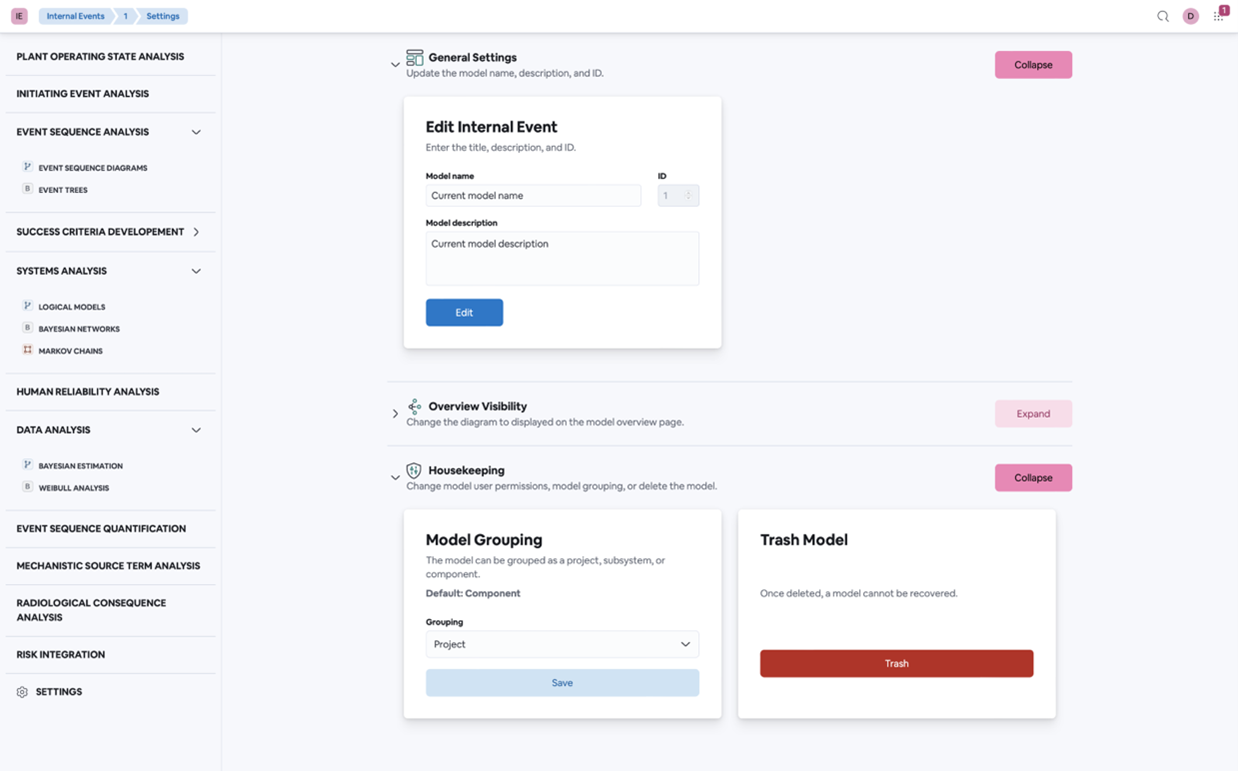
\includegraphics[width=1.0\textwidth]{4_proposed_solution/web_app/figures/analysis_modes_types.png}
  \caption{Internal events analysis overview.}
  \label{fig:analysis_modes_types}
\end{figure}

\begin{figure}
  \centering
  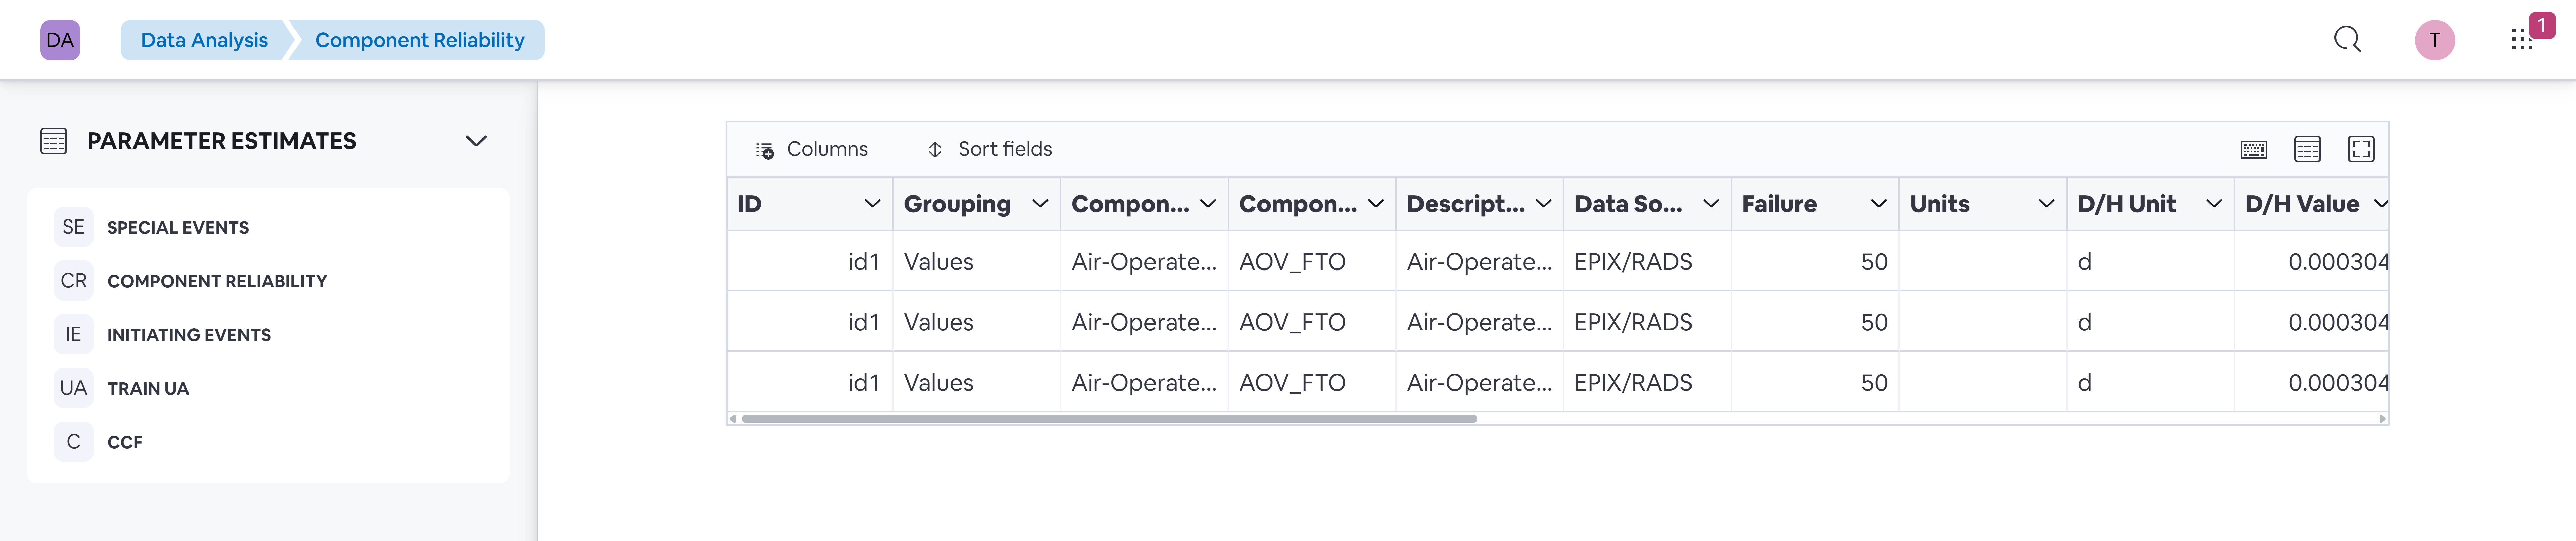
\includegraphics[width=1.0\textwidth]{4_proposed_solution/web_app/figures/data_analysis.png}
  \caption{Data analysis overview.}
  \label{fig:data_analysis}
\end{figure}

The front-end supports a wide array of risk models, each designed to address specific components of the analysis types outlined earlier. Figure \ref{fig:risk_models} shows such four risk models. 

\begin{itemize}
  \item \textbf{Initiating events:} Models and assesses potential triggers using master logic diagrams, \acrshort{fmea}, and heat balance fault trees for internal or external failures (e.g., equipment failures, human errors, natural disasters) that can shift the system into accident sequences.
  \item \textbf{Event sequence diagrams:} Provides compressed‑notation diagrams with support for cycles to model and analyze complex, temporally arranged phenomena following an initiating event.
  \item \textbf{Event trees:} Uses node and branch based diagrams to model and analyze possible sequences of events leading to specific outcomes, assessing the likelihood and consequences of each pathway.
  \item \textbf{Fault trees:} Employs Boolean gate and basic event based diagrams to model combinations of component failures and analyze their contributions to overall system failure.
  \item \textbf{Markov chains:} Applies probabilistic state transition models to analyze system reliability and availability over time through discrete states and transitions.
  \item \textbf{Bayesian networks:} Constructs directed graph models of probabilistic dependencies to analyze uncertain variables and their interactions within complex systems.
  \item \textbf{Probabilistic model checkers:} Integrates dual‑graph error propagation models to model and analyze the propagation of faults, errors, and failures through a cyber‑physical system.
  \item \textbf{Consequence models:} Links end states of event sequences with categorized outcomes (e.g., radiological doses, financial losses) and integrates them into frequency‑consequence curves for comprehensive risk evaluation.
\end{itemize}

%--------------------------------------------------------------
\begin{figure}
  \centering
  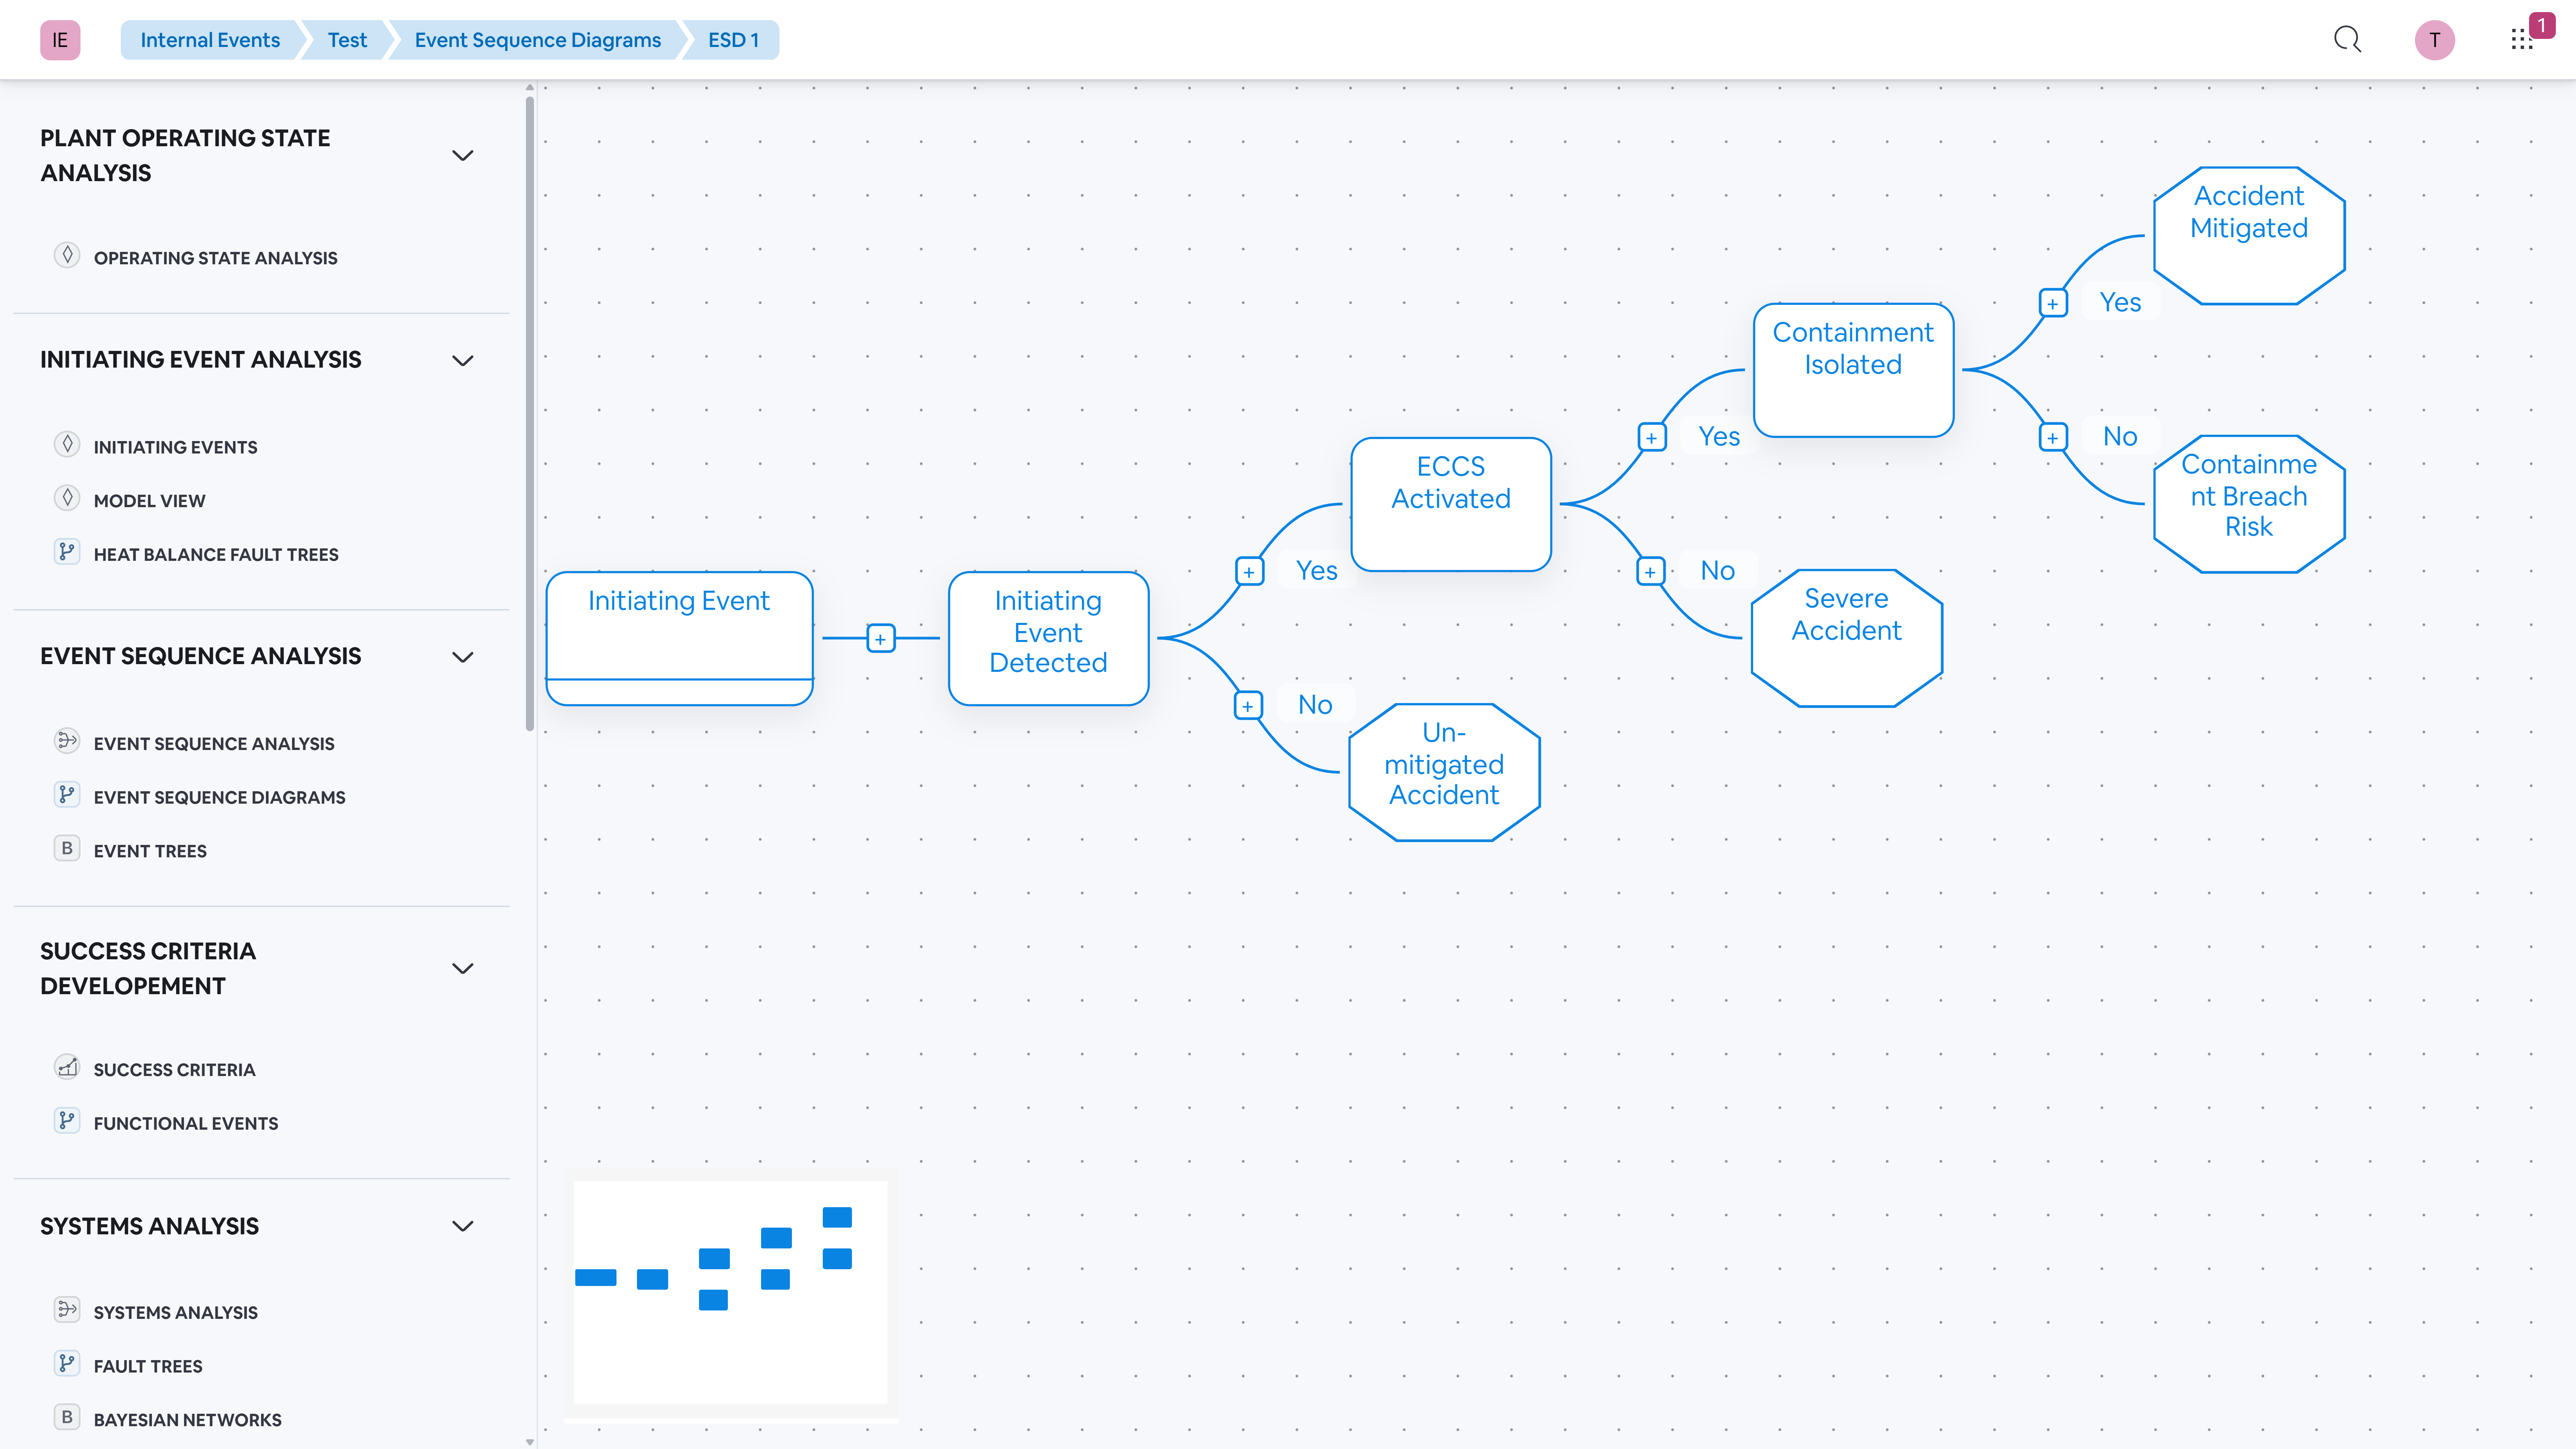
\includegraphics[width=\textwidth]{4_proposed_solution/web_app/figures/esd.png}
  \caption{Event sequence diagram editor.}
  \label{fig:esd_editor}
\end{figure}

%--------------------------------------------------------------
\begin{figure}
  \centering
  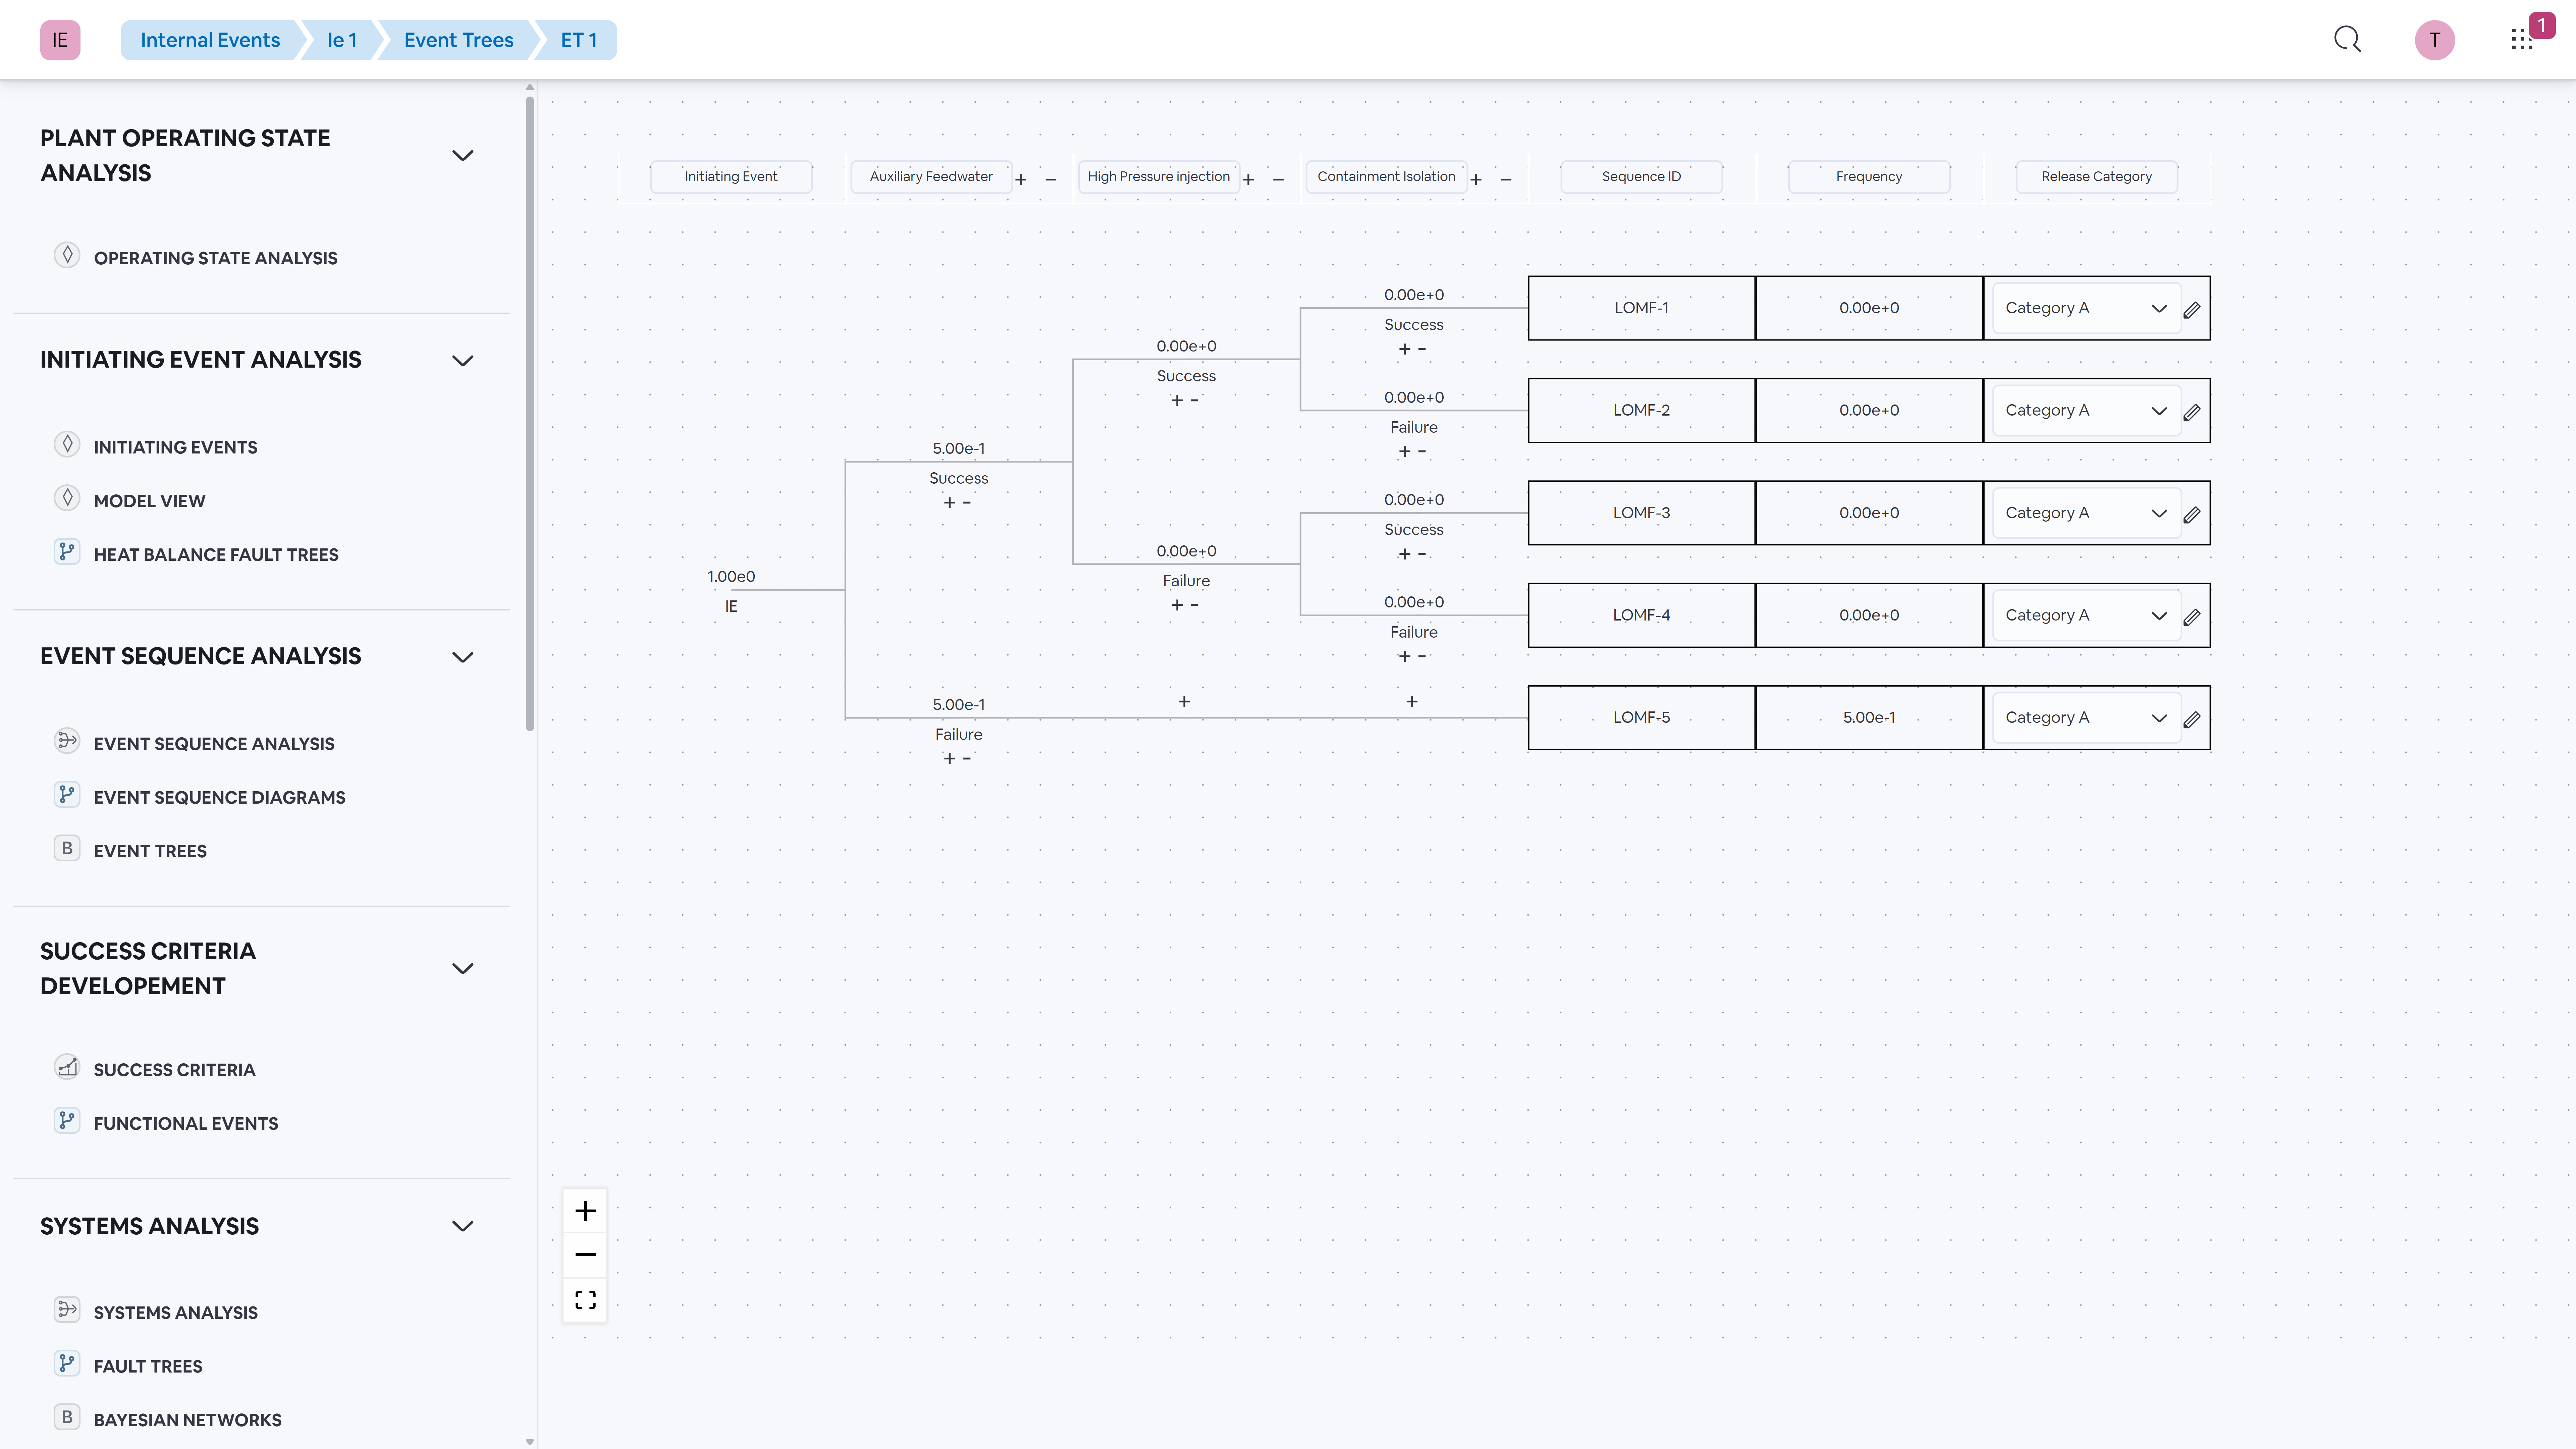
\includegraphics[width=\textwidth]{4_proposed_solution/web_app/figures/et.png}
  \caption{Event tree editor.}
  \label{fig:et_editor}
\end{figure}

%--------------------------------------------------------------
\begin{figure}
  \centering
  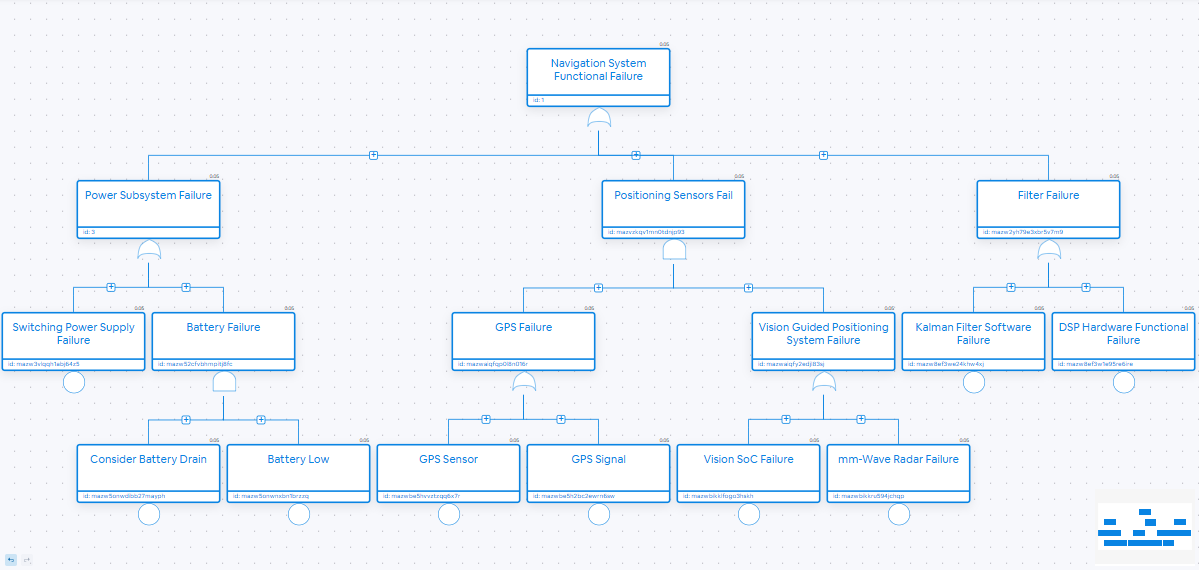
\includegraphics[width=\textwidth]{4_proposed_solution/web_app/figures/ft.png}
  \caption{Fault tree editor.}
  \label{fig:ft_editor}
\end{figure}

%--------------------------------------------------------------
\begin{figure}
  \centering
  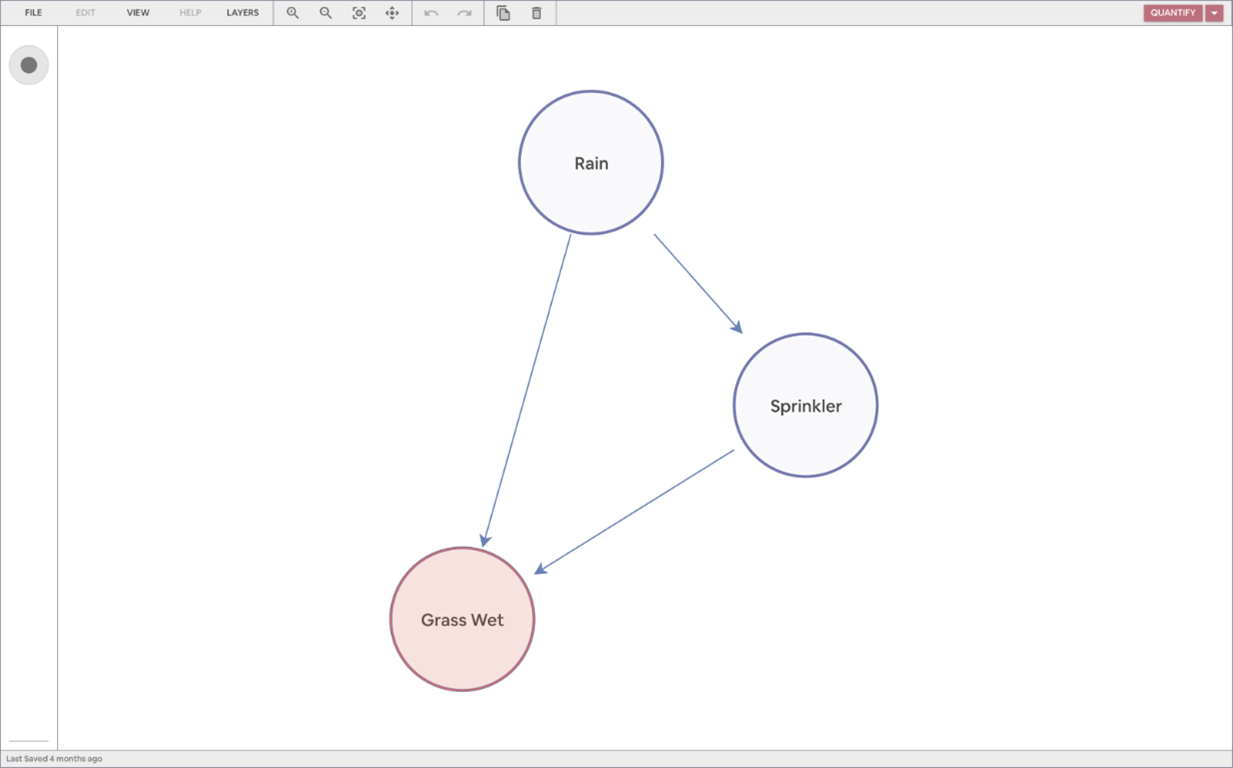
\includegraphics[width=\textwidth]{4_proposed_solution/web_app/figures/bn.png}
  \caption{Bayesian network editor.}
  \label{fig:bn_editor}
\end{figure}

OpenPRA currently uses \acrshort{hcla} as its default analyzer but is transitioning to the scram engine, with plans to phase out \acrfull{hcla} due to its proprietary license. To support advanced users, developers, and industry partners, OpenPRA offers \acrfull{api}s, tooling, and integration guides for adding custom or third‑party engines enabling on‑premise deployments and accommodating specific licensing requirements. Users can choose among multiple quantification engines when solving risk models. The front‑end provides interfaces for the following solvers:

\begin{itemize}
  \item \textbf{scram:} A command‑line tool for quantifying models specified in the OpenPSA \acrshort{mef} \acrshort{xml} schema. It implements \acrshort{bdd} for exact probability calculations, \acrshort{mocus}, along with \acrshort{mcub} and \acrshort{rea}, and \acrshort{zdd}, and supports uncertainty analysis via Monte Carlo simulation, importance analysis, and common cause failure groups (CCFGs).
  \item \textbf{XFTA:} Provides advanced fault tree quantification algorithms including cut‑set enumeration, \acrshort{mcs} generation, and importance analysis and implements \acrshort{bdd}, \acrshort{mocus}, and \acrshort{zdd} in version 2 and above.
  \item \textbf{Saphsolve:} The proprietary engine behind \acrshort{saphire}, supporting event tree analysis, fault tree analysis, and uncertainty analysis through its suite of quantification algorithms.
  \item \textbf{PRAQuant:} The default, proprietary fault tree quantification engine in Phoenix Architect, optimized for detailed fault tree analysis.
  \item \textbf{FTREX:} An optional, proprietary Phoenix Architect engine for fault tree quantification that offers additional algorithm choices.
  \item \textbf{Custom quantification engines:} Enables users to develop and integrate custom engines written in C++, Python, Java, etc. via OpenPRA’s \acrfull{api}s, allowing tailored quantification workflows.
\end{itemize}

\begin{figure}[h!]
  \centering
  \begin{subfigure}[b]{0.49\textwidth}
    \centering
    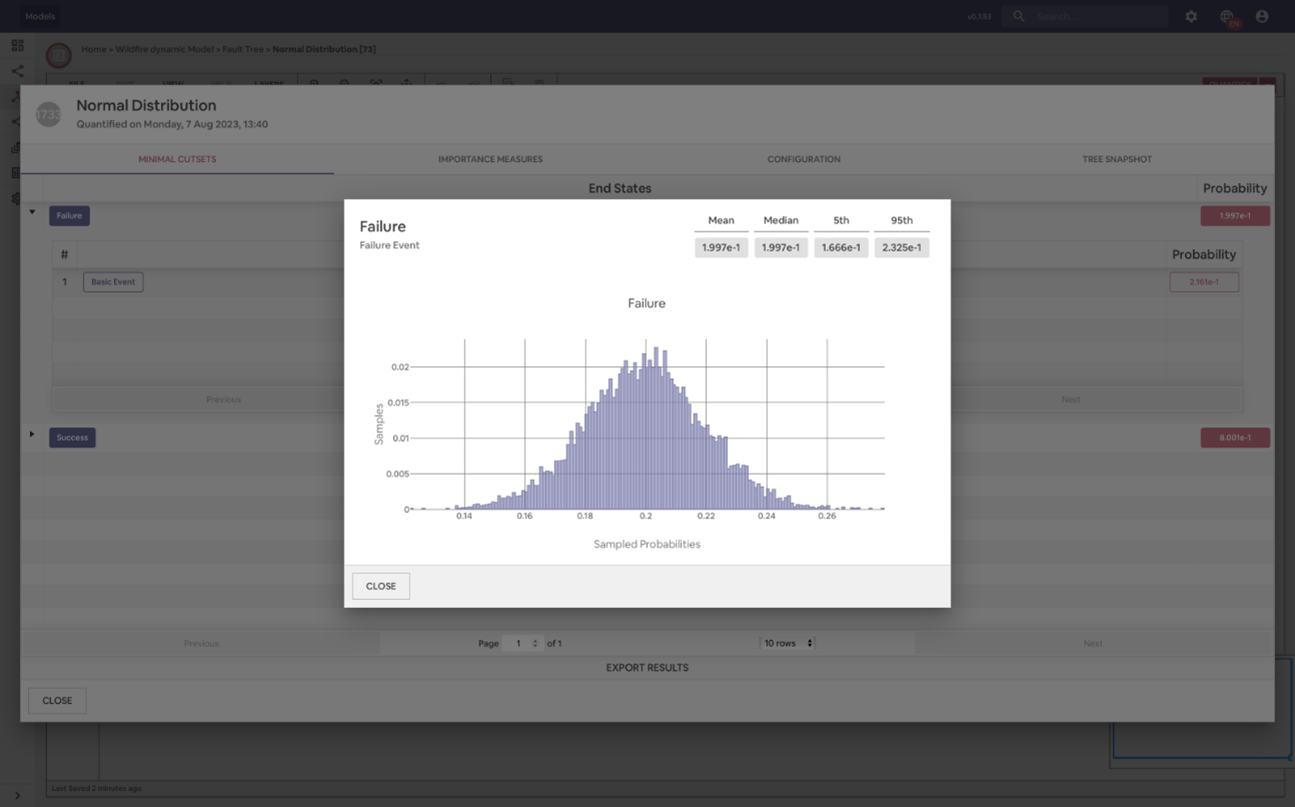
\includegraphics[width=\textwidth]{4_proposed_solution/web_app/figures/cutsets_uncertainty.png}
    \caption{}
  \end{subfigure}
  \begin{subfigure}[b]{0.49\textwidth}
    \centering
    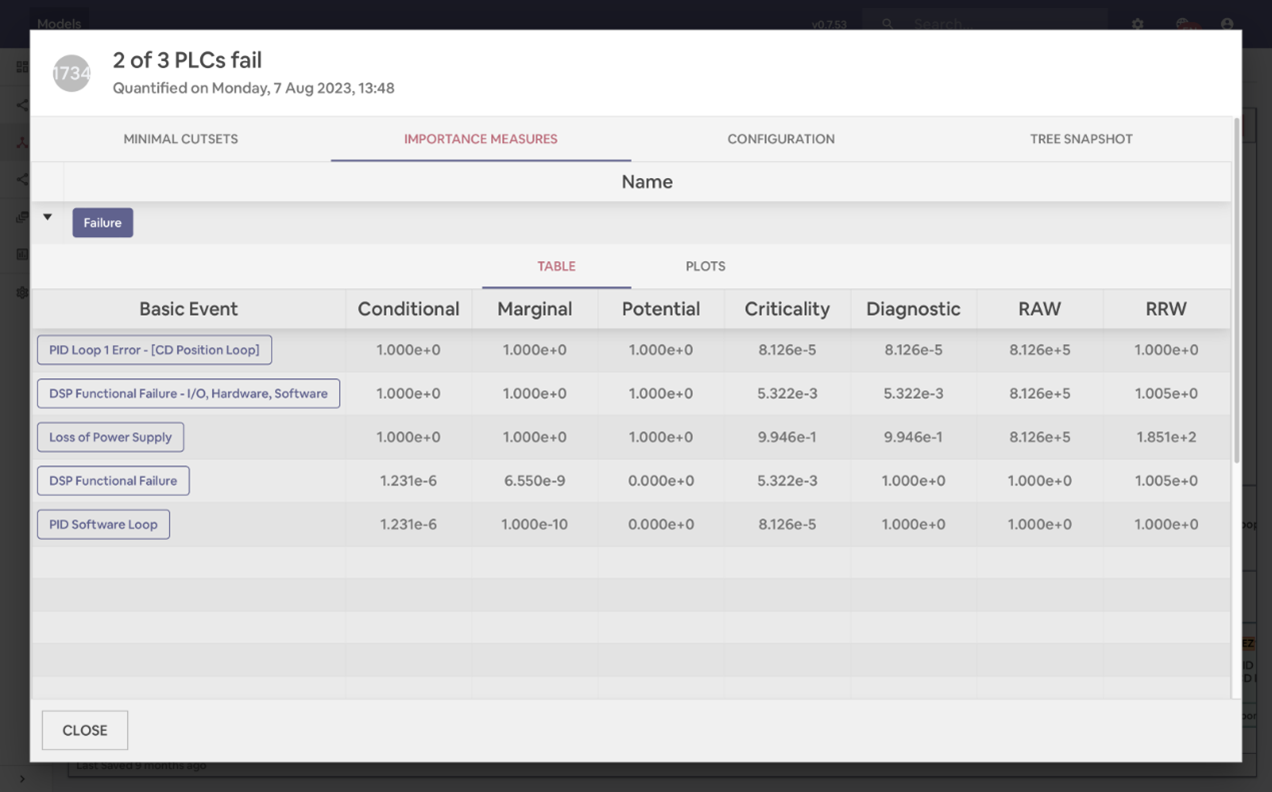
\includegraphics[width=\textwidth]{4_proposed_solution/web_app/figures/importance.png}
    \caption{}
  \end{subfigure}
  \begin{subfigure}[b]{0.49\textwidth}
    \centering
    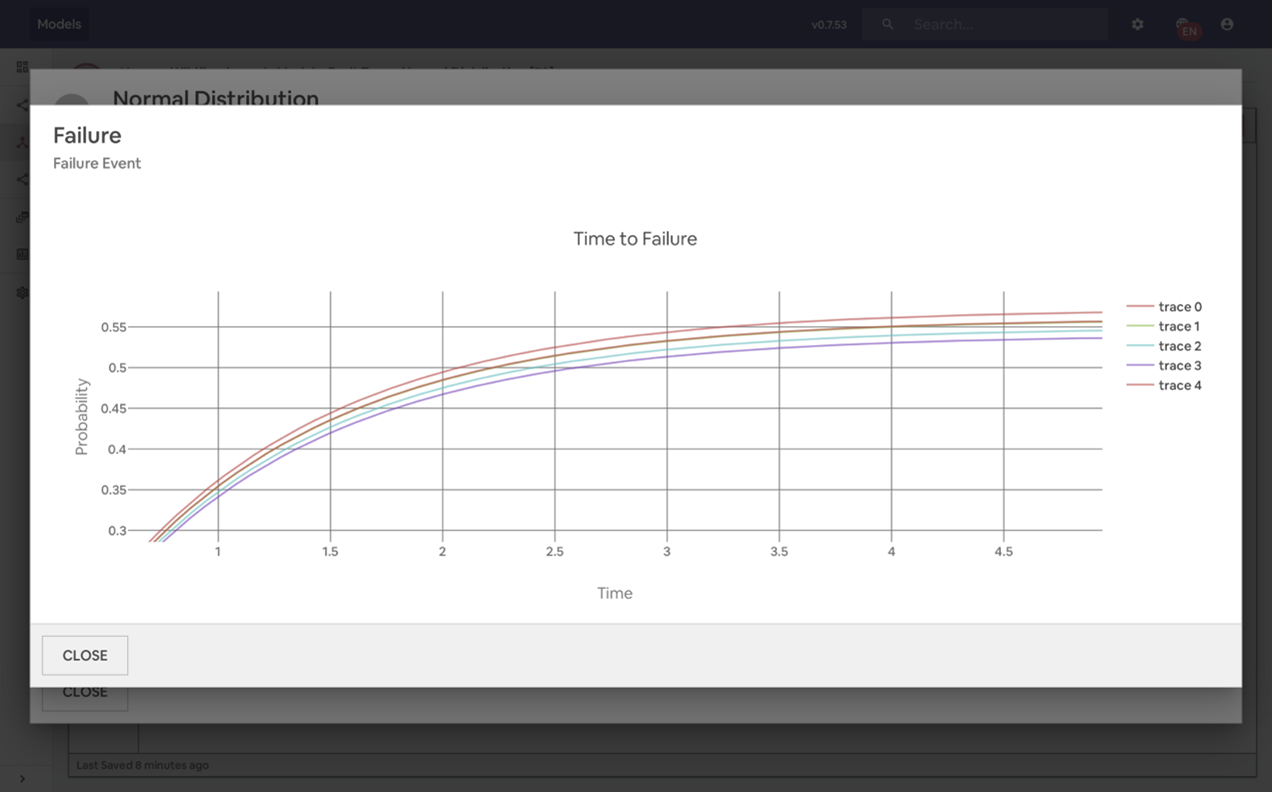
\includegraphics[width=\textwidth]{4_proposed_solution/web_app/figures/ttf.png}
    \caption{}
  \end{subfigure}
  \caption{(a) Cut sets, uncertainty using Monte Carlo sampling, (b) Importance measures calculation, (c) Time to failure cumulative distribution function with uncertainty quantification.}
  \label{fig:quantification_results}
\end{figure}

\subsection{OpenPRA Model Exchange Format}

A standardized \acrfull{mef} is critical for collaborative development, model reuse, and interoperability among \acrshort{pra} tools.  By defining a common \acrshort{json} schema, users and different tools can exchange \acrshort{pra} models without ambiguity.  \acrshort{json} was chosen over \acrshort{xml} to align with modern web technologies and simplify data handling in JavaScript/TypeScript based applications. \acrshort{json} is more compact, easier to validate, and integrates directly with the front-end and backend code.  To preserve continuity with existing \acrshort{pra} models, the format remains compatible with the legacy OpenPSA \acrshort{mef} \acrshort{xml} format via automated conversion.

The \acrshort{mef} schema provides a single, consistent definition of \acrshort{pra} models for both the OpenPRA front‑end and backend. All user input in the web editor must conform to this schema, and the backend validates the submitted \acrshort{json} against it before processing ensuring alignment with the Non‑\acrshort{lwr} \acrshort{pra} technical elements specified in \acrshort{nrc} Reg Guide 1.247.

The \acrshort{mef} schema is organized into namespaces corresponding to each of the Reg Guide 1.247 technical elements.  Each namespace defines the specific entities and attributes for that element, along with references linking it to other elements. The major namespaces include:

\begin{itemize}
  \item \textbf{Plant operating states analysis}: It defines each operating state with attributes such as power level, reactor coolant system configuration, equipment status, barrier status etc.  This namespace lists each state as a structured record.  It supports traceability by linking each state to applicable initiating events and to success criteria via ID references, ensuring that every scenario is evaluated under the correct operating conditions.
  \item \textbf{Initiating event analysis}: It defines initiating event families and individual events (internal or external hazards), along with their estimated frequencies.  Entities include grouped event definitions with triggers and fault modes.  This namespace enforces consistency by linking events to the relevant operating states (each event is associated with a POS) and by requiring presence of all mandated event categories, which ensures a complete and consistent event definition.
  \item \textbf{Event sequence analysis}: It defines event sequences (analogous to event trees) that capture the progression of system successes and failures.  Entities include sequence definitions with branching logic and outcome states.  The schema supports traceability by connecting each sequence to its initiating event, its associated success criteria, and its end states, enabling end-to-end linkage of the sequence logic across \acrshort{pra} elements.
  \item \textbf{Success criteria development}: It defines the success criteria for safety functions and systems given specific initiating events.  Entities include criteria records that list the required systems, components, and actions needed to meet each safety function.  The schema ties each success criterion to corresponding system or component IDs and to event sequences, ensuring that every criterion is linked to the relevant events and system configurations.
  \item \textbf{Systems analysis}: It defines system models including components, failure modes, subsystem dependencies, and common-cause failures.  Entities include system topology and fault tree structures for system unavailability.  It supports quantification by explicitly declaring component IDs and failure relationships, enabling automated checking of dependency effects (e.g.\ CCFs) and completeness of the system model.
  \item \textbf{Human reliability analysis}: Implements the Human Reliability Analysis element.  It defines \acrfull{hfe}s, task descriptions, and recovery actions.  Entities include \acrshort{hfe} definitions linked to plant states, system conditions, and operator actions.  It provides traceability by associating each \acrshort{hfe} with the specific plant state and system context in which it can occur, ensuring that all human errors are connected to the relevant event sequences.
  \item \textbf{Mechanistic source term analysis}: It defines release categories and source-term parameters for radioactive material releases.  Entities include source-term models (e.g.\ fractions of radionuclides released) tied to specific sequences and physical barriers.  The schema supports quantification by linking each release category back to its triggering event sequence and to the success criteria, enabling consistent calculation of source terms.
  \item \textbf{Radiological consequence analysis}: It defines consequence calculation scenarios, dose endpoints, and transport pathways.  Entities include consequence cases that map release quantities to dose or risk metrics.  It captures dependencies by connecting each consequence case to the corresponding release category from the source-term analysis and to plant conditions, so that material releases are systematically propagated to dose outcomes.
  \item \textbf{Risk integration}: It defines the aggregated \acrshort{pra} model, including top events, cut sets, and risk metrics.  Entities include combined risk data structures and summary outputs.  It provides end-to-end traceability by linking each calculated frequency or risk value back to the contributing initiating events, sequences, systems, and success criteria, ensuring that the entire \acrshort{pra} chain is connected.
\end{itemize}

\subsection{Backend \acrshort{rest} \acrshort{api}}

The OpenPRA backend is a Node.js based \acrshort{rest} \acrshort{api} that coordinates all qualitative \acrshort{pra} workflows, exposing \acrfull{crud} endpoints for every element defined by the OpenPRA \acrfull{mef} schema. Contrary to the distributed job system's \acrshort{rest} \acrshort{api}, which is an independent microservice dedicated to quantification operations only, the backend \acrshort{rest} \acrshort{api} is tightly integrated with the web front‑end and the distributed databases. Thus, computational requests are routed to the job broker’s \acrshort{api}, while model editing, security, and user management operations are handled by the backend \acrshort{api}. All client requests from the front-end go through this \acrshort{api}, which handles user authentication, authorization, and persists model data in the distributed databases. In practice, each \acrshort{mef} namespace has a corresponding set of \acrshort{api} routes. For example, endpoints such as \texttt{`/api/fault-trees`} or \texttt{`/api/event-trees`} allow clients to create, read, update, or delete the graph-structured \acrshort{pra} models.  The front‑end data is first validated by the Nestia runtime library against the OpenPRA \acrshort{mef} \acrshort{json} schema and then they are saved as \acrfull{bson} documents inside the database.

The backend implements full user and collaboration management.  It provides endpoints for user registration, login (issuing JWT tokens), password verification, and user profile or solver preferences.  It secures these endpoints using JWT/OAuth2 guards and role-based access control. Role and invitation endpoints allow administrators to create new roles, assign permissions, and manage team collaboration (including sending or verifying invitation tokens for new users).  

Table \ref{tab:openpra-backend-endpoints} lists the main \acrshort{api} entry points (grouped by function), with the \acrshort{http} request methods they support and a brief description of each endpoint’s purpose:

\begin{landscape}
\begin{longtable}{@{}lll@{}}
\caption{Main REST API entrypoints exposed by the OpenPRA backend.}
\label{tab:openpra-backend-endpoints}\\
\toprule
\textbf{Endpoint} & \textbf{Methods} & \textbf{Description} \\
\midrule
\endfirsthead
\multicolumn{3}{c}{\textit{Continued: Main REST API entrypoints exposed by the OpenPRA backend.}}\\
\toprule
\textbf{Endpoint} & \textbf{Methods} & \textbf{Description} \\
\midrule
\endhead
\bottomrule
\endfoot
%
\multicolumn{3}{@{}l}{\textbf{Authentication}}\\
\midrule
\texttt{/api/auth/token-obtain} & POST & Issue JWT token (user login) \\
\texttt{/api/auth/verify-password} & POST & Verify user credentials/password \\
\addlinespace
\multicolumn{3}{@{}l}{\textbf{Collaboration (Users)}}\\
\midrule
\texttt{/api/collab/user} & GET, POST & List users; create new user \\
\texttt{/api/collab/user/\{user\_id\}} & GET, PUT & Get or update a user by ID \\
\texttt{/api/collab/user/\{user\_id\}/preferences} & GET, PUT & Get or update user preferences \\
\texttt{/api/collab/validateEmail} & POST & Check email availability/validity \\
\texttt{/api/collab/validateUsername} & POST & Check username uniqueness \\
\addlinespace
\multicolumn{3}{@{}l}{\textbf{Collaboration (Invites \& Roles)}}\\
\midrule
\texttt{/api/collab/invite} & POST, PUT & Create or update an invitation \\
\texttt{/api/collab/invites} & GET & List all invitations \\
\texttt{/api/collab/invite/\{id\}} & GET, DELETE & Get or cancel invite by ID \\
\texttt{/api/collab/verify-invite} & POST & Verify/redeem an invite token \\
\texttt{/api/collab/roles} & GET, POST, PUT & List, create, or update access roles \\
\texttt{/api/collab/roles/\{roleId\}} & DELETE & Delete a role by ID \\
\addlinespace
\multicolumn{3}{@{}l}{\textbf{Model Graphs}}\\
\midrule
\texttt{/api/model/fault-tree-graph} & GET, POST & Create or retrieve fault-tree graph structure \\
\texttt{/api/model/event-tree-graph} & GET, POST & Create or retrieve event-tree graph structure \\
\texttt{/api/model/event-sequence-diagram-graph} & GET, PATCH & Get or update event-sequence diagram graph \\
\texttt{/api/model/event-sequence-diagram-graph/update-label} & PATCH & Update labels on the event-sequence graph \\
\addlinespace
\multicolumn{3}{@{}l}{\textbf{\acrfull{fmea}}}\\
\midrule
\texttt{/api/model/fmea/\{id\}} & GET & Retrieve FMEA table by ID \\
\texttt{/api/model/fmea/\{id\}/row} & PUT & Add or update a row in the FMEA \\
\texttt{/api/model/fmea/\{id\}/column} & PUT & Add or update a column in the FMEA \\
\texttt{/api/model/fmea/\{id\}/cell} & PUT & Update a cell value in the FMEA \\
\texttt{/api/model/fmea/\{id\}/dropdown} & PUT & Update dropdown options in the FMEA \\
\texttt{/api/model/fmea/\{id\}/delete} & PUT & Delete the entire FMEA table \\
\texttt{/api/model/fmea/\{id\}/column/updateName} & PUT & Rename a FMEA column \\
\texttt{/api/model/fmea/\{id\}/column/updateType} & PUT & Change a column’s type \\
\texttt{/api/model/fmea/\{fmeaid\}/\{rowid\}/delete} & DELETE & Delete a specific FMEA row \\
\addlinespace
\multicolumn{3}{@{}l}{\textbf{Typed Models (Hazard Tables)}}\\
\midrule
\texttt{/api/model/internal-events} & GET, POST, DELETE & Manage internal-event entries \\
\texttt{/api/model/internal-events/\{id\}} & GET, PATCH & Get or update an internal-event by ID \\
\texttt{/api/model/internal-hazards} & GET, POST, DELETE & Manage internal-hazard entries \\
\texttt{/api/model/internal-hazards/\{id\}} & GET, PATCH & Get or update an internal-hazard by ID \\
\texttt{/api/model/external-hazards} & GET, POST, DELETE & Manage external-hazard entries \\
\texttt{/api/model/external-hazards/\{id\}} & GET, PATCH & Get or update an external-hazard by ID \\
\texttt{/api/model/full-scope} & GET, POST, DELETE & Manage full-scope analysis entries \\
\texttt{/api/model/full-scope/\{id\}} & GET, PATCH & Get or update a full-scope entry by ID \\
\addlinespace
\multicolumn{3}{@{}l}{\textbf{Other PRA Components}}\\
\midrule
\texttt{/api/model/initiating-events} & POST & Add initiating events to a model \\
\texttt{/api/model/markov-chains} & POST & Add Markov chain models \\
\texttt{/api/model/weibull-analysis} & POST & Add Weibull failure-rate data \\
\texttt{/api/model/risk-integration} & POST & Add risk integration parameters \\
\texttt{/api/model/radiological-consequence-analysis} & POST & Add consequence-model data \\
\texttt{/api/model/mechanistic-source-term} & POST & Add source-term model data \\
\texttt{/api/model/event-sequence-quantification-diagram} & POST & Add event-sequence quantification diagrams \\
\texttt{/api/model/data-analysis} & POST & Add data-analysis entries \\
\texttt{/api/model/human-reliability-analysis} & POST & Add HRA entries \\
\texttt{/api/model/systems-analysis} & POST & Add systems analysis entries \\
\texttt{/api/model/success-criteria} & POST & Add success-criteria entries \\
\texttt{/api/model/event-sequence-analysis} & POST & Add event-sequence analysis entries \\
\texttt{/api/model/operating-state-analysis} & POST & Add operating-state analysis entries \\
\addlinespace
\multicolumn{3}{@{}l}{\textbf{Quantification}}\\
\midrule
\texttt{/api/quantify/with-scram-binary} & POST & Submit a model to the SCRAM engine via job queue \\
\end{longtable}
\end{landscape}


\subsection{Distributed Databases}

Distributed, \acrshort{nosql} document databases provide a scalable and flexible backend for storing and managing both the structure of \acrshort{pra} models and the results of risk analyses. These databases (e.g.\ MongoDB containers deployed through Docker swarm) allow complex hierarchical model data including fault trees, event trees, Markov chains, initiating event analyses, component reliability parameters, and quantification results to be stored as \acrshort{bson} documents. By replicating data across multiple nodes, the database ensures high availability and fault tolerance for critical risk information. Through indexing and querying, users can search and aggregate model components (e.g.\ summarizing risk metrics across scenarios). In this way,the distributed database orchestrates the entire data management layer of the application, enabling large-scale \acrshort{pra} models to be persistently stored and quickly accessed by web clients and analysis engines.

\subsubsection{OpenPRA \acrshort{mef} Persistence}

OpenPRA uses MongoDB to persist structured model data according to the OpenPRA \acrshort{mef} \acrshort{json} schema. MongoDB’s document model naturally represents nested \acrshort{pra} data: for instance, an entire fault tree or its branches can be stored as an embedded document, and arrays of events or transitions can be stored directly within a model document. \acrshort{crud} operations are efficiently handled by MongoDB’s native \acrshort{api}. For example, when a user edits a model (e.g., by adding a gate to a fault tree), the application atomically updates the corresponding MongoDB document without sending the entire fault tree structure. Indexed fields in the database ensure that queries (such as looking up a specific event by its ID) are executed quickly.

\subsubsection{Version Control and Revision History}

The database enables version control of models. Every change to a model can be tagged with a revision identifier, timestamp, and author, and full snapshots of the model state can be recorded in the database. OpenPRA can store each committed version of a model as a separate document, allowing users to roll back to any previous state and inspect differences between revisions.

\subsubsection{Sharding for Scalability}

Sharding partitions a collection across multiple servers based on a shard key (for example, a model ID). This means, different parts a model such as different sub-trees of a model can reside on different shards. Queries targeting a particular model are routed to the correct shard, distributing the query load. This horizontal partitioning allows storage and processing of very large structures (such as nested event trees or high order Markov chains) beyond what a single MongoDB document can hold.

\subsubsection{Support for Dynamic Schema}

MongoDB does not require a fixed data structure, so different documents can have different data types and fields. OpenPRA leverages this by storing varying technical elements and analyses results as distinct document types under a unified database. Validation rules can still be applied per collection to ensure that each document type conforms to an expected structure and data types. This means if new data fields or \acrshort{pra} elements are defined, the database can accommodate those changes seamlessly while still ensuring data validation.

\subsection{Key Differences from v1 to v2}
\label{sec:distinguish-v1-v2}
This subsection provides a concise overview of the differences between the original OpenPRA \textit{v1} application and the updated \textit{v2} application as developed in this study, without repeating the extensive details offered in previous sections.

\paragraph{Overview of the v1 Application}
The \textit{v1} app introduced the concept of a web-based \acrshort{pra} platform, embedding \acrshort{hcla} as its default solver. Originally, it aimed to demonstrate how an online tool could integrate event sequence diagrams, fault trees, and Bayesian networks under a single interface. However, its reliance on a largely closed-source back end and limited extensibility restricted broader collaboration and support for high-performance computing. Figure \ref{fig:quantification_results} illustrates the various types of quantification supported by HCLA.

\paragraph{Overview of the v2 Application}

\begin{comment}
The \textit{v2} update was driven by the need to improve openness, scalability, and solver flexibility. Three major goals encapsulate these objectives:
\begin{enumerate}
    \item \textbf{Architectural overhaul for extensibility and maintainability}, ensuring that new quantification methods or specialized back ends can be more easily integrated. 
    \item \textbf{Distributed computing and parallelization}, allowing a larger number of simultaneous analyses and more rigorous Monte Carlo sampling under high-throughput demands. 
    \item \textbf{Open-source licensing and community involvement}, encouraging collaboration from researchers and practitioners who can actively contribute domain-specific plug-ins or enhancements.
\end{enumerate}

\subsubsection{Architectural and Implementation Differences}
\subsubsection{Solver Integration and Model Exchange}
\subsubsection{Performance and Scalability Enhancements}
\end{comment}

The \textit{v2} system replaces the legacy monolithic application with a monorepo based architecture. The \textit{v2} codebase supports container orchestration, simplifying deployment, scaling, and maintenance. Whereas \textit{v1} ran all logic in a single back‑end process, \textit{v2} separates model editing services from resource intensive solver workloads by offloading computations to a distributed job queue managed by a dedicated broker. In place of the earlier SQL database, \textit{v2} employs a fully distributed NoSQL datastore with advanced sharding, enabling efficient storage and retrieval of large‑scale PRA models and analysis results.

Whereas \textit{v1} depended on the proprietary \acrshort{hcla} engine for quantification, \textit{v2} adopts the open‑source \texttt{scram} solver as its default, eliminating barriers that previously hindered external collaboration. The new architecture also supports modular plug‑ins for alternative engines such as \texttt{XFTA}, \texttt{Saphsolve} etc. so that teams can choose solvers that match their modeling paradigms or licensing requirements. Complementing this extensibility, \textit{v2} introduces a more flexible schema that ensures interoperability with third party tools and enforces consistent data validation across the platform.

While \textit{v1} app handled quantification operations adequately for single‑user or light workloads, \textit{v2} app is engineered for high throughput under concurrent use. It is capable of executing multiple large models in parallel and thereby shortening overall runtimes. It can also leverage optional GPU acceleration and multi‑core CPU strategies such as data‑parallel Monte Carlo sampling and parallel computing algorithms to speed up advanced tasks like probability and uncertainty estimation.

Finally, \textit{v2} has transitioned away from the restricted licensing of \textit{v1} toward a more open development model. \textit{v2} encourages researchers and industry experts to customize and expand the code base. \textit{GitHub} or comparable platforms host the source code, enabling issue tracking, pull requests, and community plugins. The switch to open licensing simplifies collaborative usage of the newly introduced \acrshort{json}-based \acrshort{mef} for exchanging models globally.